\documentclass{slides}

\usepackage[ngerman]{babel}
\usepackage{array}
\usepackage{tikz}

\lstset{language=C}

%%%%%%%%%%%%%%%%%%%%%%%%%%%%%%%%%%%%%%%%%%%%%%%%%%%%%%%%%%%%%%%%%%%%%%%%%

\begin{document}

\graphicspath{{figures/}}

\title[Programming in C++]{\Large Programming in C++}

\author[A. Arnold and O. Lenz]{Axel Arnold \and Olaf Lenz} 
\institute{Institut für Computerphysik\\Universit\"at Stuttgart}
\date{February 18-22, 2013}

\setbeamertemplate{footline}{}
\begin{frame}
  \titlepage
\end {frame}
\setbeamertemplate{footline}[icp]

\begin{frame}
  \frametitle{Die Compilersprache C}

  \begin{columns}[c,onlytextwidth]
    \column{0.5\textwidth}
    \centering
    
\includegraphics[height=0.25\textheight]{ritchie}\\
    {\small D. M. Ritchie, 1941 -- 2011}

    \column{0.5\textwidth}
    \centering
    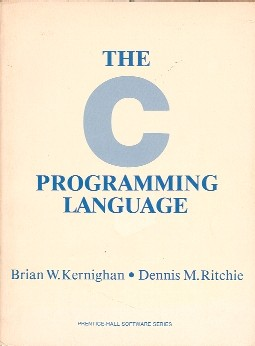
\includegraphics[height=0.35\textheight]{kr-c}
  \end{columns}
  \vspace{0.5em}


  \only<1>{
    \minisec{Geschichte}
    \vspace{0.5em}

    \begin{tabular}{r<{:}l}
      1971-73 & Entwickelt von D. M. Ritchie\\
      1978 & C-Buch von Kernighan und Ritchie ("`K\&R-C"')\\
      1989 & Standard ANSI C89 = ISO C90\\
      1999 & Standard ISO C99 (im folgenden benutzt)
    \end{tabular}
  
    \begin{itemize}
    \item Zur Zeit Arbeiten am nächsten Standard, C1X
    \item Außerdem Compiler-spezifische Erweiterungen
    \item Objektorientierte Programmierung: Objective-C, C++
    \end{itemize}
  }
  \only<2>{
    \minisec{C-Compiler}
    \begin{itemize}
    \item übersetzt C-Quellcode in Maschinencode
    \item GNU gcc, Intel icc, IBM XL C, Portland Group Compiler, ...
    \item Für praktisch alle Prozessoren gibt es C-Compiler
    \item Compiler optimieren den Maschinencode
    \item Compiler übersetzt nur Schleifen, Funktionsaufrufe usw.
    \item Bibliotheken für Ein-/Ausgabe, Speicherverwaltung usw.
    \end{itemize}
  }
  \only<3>{
    \minisec{Einsatzgebiete}
    \begin{itemize}
    \item C ist geeignet für effiziente und hardwarenahe Programme
    \item alle modernen Betriebssystem-Kernel sind in C geschrieben
    \item Der Python-Interpreter ist in C geschrieben
    \item Gnome oder KDE sind größtenteils C/C++-Code
    \item Viele physikalische Software ist C (oder Fortran)
    \end{itemize}
  }
  \only<4>{
    \minisec{Eigenschaften}
    \begin{itemize}
    \item C-Code oft deutlich schneller als z.B. Python-Code
    \item Besonders bei numerischen Problemen
    \item Intensiver Einsatz von Zeigern
    \item Kein Schutz gegen Speicherüberläufe
    \item Erzeugter Maschinencode schwer zu verstehen
    \end{itemize}
  }
\end{frame}

\begin{frame}[fragile]
  \frametitle{Hello, World!}

  \only<2>{\lstset{emph={int,main}}}
  \only<3>{\lstset{emph={return}}}
  \only<4>{\lstset{emph={printf,include,stdio.h}}}
  \only<5>{\lstset{emph={include}}}
  \begin{lstlisting}
#include <stdio.h>

int main()
{
  printf("Hello, World\n");
  return 0;
}
\end{lstlisting}
  \lstset{emph={}}

  \begin{onlyenv}<1>
    \begin{itemize}
    \item C-\alert{Quellcode} muss als Textdatei vorliegen (z.B. \lstinline!helloworld.c!)
    \item Vor der Ausführung mit dem GNU-Compiler \alert{compilieren}:
\begin{lstlisting}[frame={},language=bash]
gcc -Wall -O3 -std=c99 -o helloworld helloworld.c
\end{lstlisting}
    \item Erzeugt ein \emph{Binär}programm \lstinline!helloworld!,\\
      d.h. das Programm ist betriebssystem- und architekturspezifisch
    \item "`-Wall -O3 -std=c99"' schaltet bei gcc alle Warnungen und die Optimierung an,
      und wählt den ISO C99-Standard anstatt C90
    \end{itemize}
  \end{onlyenv}

  \begin{onlyenv}<2>
    \begin{itemize}
    \item \lstinline!main! ist eine selbstdefinierte \alert{Funktion}
    \item Hier startet das Programm, daher muss es \lstinline!main! immer geben
    \item Rückgabewert vom \alert{Datentyp} \lstinline!int!
    \item Keine Parameter ("`\lstinline!()!"')
    \item Code der Funktion: Block in geschweiften Klammern
    \item Anweisungen werden mit Semikolon beendet
    \end{itemize}
  \end{onlyenv}

  \begin{onlyenv}<3>
    \begin{itemize}
    \item {\alerted\lstinline!return!} beendet die Funktion \lstinline!main!
    \item Argument von \lstinline!return! ist der Rückgabewert der Funktion (hier 0)
    \item Der Rückgabewert von \lstinline!main! geht an die Shell,\\
      vergleiche \lstinline!exit! in bash oder Python
    \end{itemize}
  \end{onlyenv}

  \begin{onlyenv}<4>
    \begin{itemize}
    \item \lstinline!printf! ist eine Bibliotheksfunktion
    \item Formatierte Textausgabe analog "`\%"' in Python
    \item Benötigt Headerdatei \texttt{"`stdio.h"'}
    \item Einbinden einer Headerdatei entspricht in etwa "`import"' in Python
    \end{itemize}
  \end{onlyenv}

  \begin{onlyenv}<5>
    \begin{itemize}
    \item \lstinline!#include! ist \alert{Präprozessor-Anweisung}
    \item Bindet den Code der \alert{Headerdatei} \lstinline!stdio.h! ein
    \item Headerdateien beschreiben Funktionen anderer Module,\\
      z.B. \lstinline!stdio.h! Ein-/Ausgabefunktionen wie
      \lstinline!printf!
    \item \lstinline!stdio.h! ist Systemheaderdatei,
      Bestandteil der C-Umgebung
    \end{itemize}
  \end{onlyenv}
\end{frame}

\begin{frame}[fragile]
  \frametitle{Formatierung}
  \vspace{-\baselineskip}

  \begin{columns}[t,onlytextwidth]
    \column{0.48\textwidth}
\begin{lstlisting}
#include <stdio.h>

int main()
{
  printf("Hallo Welt\n");
  return 0;
}
\end{lstlisting}
    \column{0.48\textwidth}
\begin{lstlisting}
#include         <stdio.h>
    int main(){printf(
"Hallo Welt\n");return 0;}
\end{lstlisting}   
  \end{columns}

  \begin{itemize}
  \item C lässt viele Freiheiten bei der Formatierung des Quelltexts
  \item Aber: falsche Einrückung erschwert Fehlersuche
    \begin{alertbox}{0.7\textwidth}
      Lesbarer C-Code erfordert Disziplin!
    \end{alertbox}
    \vspace{0.5em}

  \item Weitere Beispiele: The International Obfuscated C Code Contest\\
    \url{http://www.ioccc.org/main.html}
  \end{itemize}
\end{frame}

\begin{frame}[fragile]
  \frametitle{Datentypen in C}
  \begin{itemize}
  \item \alert{Grunddatentypen}

    \begin{center}
      \renewcommand{\arraystretch}{1.2}
      \begin{tabular}{|l|l|l|}
        \hline
        \lstinline!char! & 8-Bit-Ganzzahl, für Zeichen & '1','a','A',... \\\hline
        \lstinline!int! & 32- oder 64-Bit-Ganzzahl & 1234, -56789\\\hline
        \lstinline!float! & 32-Bit-Fließkommazahl & 3.1415, -6.023e23\\\hline
        \lstinline!double! & 64-Bit-Fließkommazahl & -3.1415, +6.023e23\\\hline
      \end{tabular}
    \end{center}

  \item \alert{Arrays} (Felder): ganzzahlig indizierter Vektor
  \item \alert{Pointer} (Zeiger): Verweise auf Speicherstellen
  \item \alert{Structs und Unions}: zusammengesetzte Datentypen, Datenverbünde
  \item {\alerted \lstinline!void!} (nichts): Datentyp, der nichts speichert
    \begin{itemize}
    \item Rückgabewert von Funktionen, die nichts zurückgeben
    \item Zeiger auf Speicherstellen unspezifierten Inhalts
    \end{itemize}
  \end{itemize}
\end{frame}

\begin{frame}[fragile]
  \frametitle{Typumwandlung}

\begin{lstlisting}
int nenner = 1;
int zaehler = 1000;
printf("Ganzzahl: %f\n",
  (float)(nenner/zaehler)); // @\textrightarrow{} 0.000000@
printf("Fliesskomma: %f\n",
  ((float) nenner)/zaehler); //@\textrightarrow{} Fliesskomma: 0.001000@
\end{lstlisting}

  \begin{itemize}
  \item C wandelt Typen nach Möglichkeit automatisch um
  \item Explizite Umwandlung: geklammerter Typname vor Ausdruck\\
    \emph{Beispiel:} \lstinline!(int)( ((float) a) / b)!
  \item Notwendig bei Umwandlung
    \begin{itemize}
    \item \lstinline!int! \ensuremath{\leftrightarrow}{} \lstinline!float!
    \item von Zeigern
    \end{itemize}
  \item Umwandlung in \lstinline!void! verwirft den Ausdruck
  \end{itemize}
\end{frame}

\begin{frame}[fragile]
  \frametitle{Variablen}

  \only<1>{\lstset{emph={global,i}}}
  \only<2>{\lstset{emph={global}}}
  \only<3>{\lstset{emph={i}}}

\begin{onlyenv}<1-3>
\begin{lstlisting}
int global;
int main() {
  int i = 0, j, k;
  global = 2;
  int i;  // Fehler! i doppelt deklariert
}
void funktion() {
  int i = 2; // Ok, da anderer Gueltigkeitsbereich
  i = global;
}
\end{lstlisting}
  \lstset{emph={}}
\end{onlyenv}

  \begin{onlyenv}<1>
    \alert{Variablen}
    \begin{itemize}
    \item \emph{müssen} vor Benutzung mit ihrem Datentyp \alert{deklariert} werden
    \item dürfen \emph{nur einmal} deklariert werden
    \item können bei der Deklaration mit Startwert \alert{initialisiert} werden
    \item Mehrere Variablen desselben Typs mit "`,"' getrennt deklarieren
    \end{itemize}
  \end{onlyenv}

  \begin{onlyenv}<2>
    \minisec{Globale Variablen}
    \begin{itemize}
    \item hier: Die Ganzzahl \lstinline!global!
    \item Deklaration außerhalb von Funktionen
    \item Aus allen Funktionen les- und schreibbar
    \end{itemize}
  \end{onlyenv}
  \begin{onlyenv}<3>
    \minisec{Lokale Variablen}
    \begin{itemize}
    \item hier: Die Ganzzahl \lstinline!i!
    \item Gültigkeitsbereich ist der innerste offene Kontext (Block)
    \item daher kann \lstinline!i! in \lstinline!main! und \lstinline!funktion!
      deklariert werden
    \end{itemize}
  \end{onlyenv}
\end{frame}

\begin{frame}[fragile]
  \frametitle{Bedingte Ausführung -- if}
\begin{lstlisting}
if (anzahl == 1) { printf("ein Auto\n"); }
else             { printf("%d Autos\n", anzahl); }
\end{lstlisting}

  \begin{itemize}
  \item \lstinline!if! wie in Python
  \item Es gibt allerdings kein \lstinline!elif!
  \end{itemize}
  \vfill

  \begin{block}{Bedingungen}
    Ähnlich wie in Python, aber
    \begin{itemize}
    \item logisches "`und"': "`\&\&"' statt "`and"'
    \item logisches "`oder"': "`||"' statt "`or"'
    \item logisches "`nicht"': "`!"' statt "`not"'
    \end{itemize}
    Also z.B.: \lstinline/  !((a == 1) || (a == 2))/
  \end{block}
\end{frame}

\begin{frame}[fragile]
  \frametitle{Schleifen -- for}

  \begin{onlyenv}<1>
\begin{lstlisting}
for (@\color{CDred}int i = 1@; @\color{CDgreen} i < 100@; @\color{CDblue1} ++i@) {
  printf("%d\n", i);
}
for (@\color{CDred}int k = 100@; @\color{CDgreen} k > 0@; @\color{CDblue1} k /= 2@)
  printf("%d\n", k);
\end{lstlisting}

    \lstinline!for!-Schleifen bestehen aus
    \begin{itemize}
    \item \textcolor{CDred}{Initialisierung der Schleifenvariablen}\\
      \begin{itemize}
      \item Eine hier deklarierte Variable ist nur in der Schleife gültig
      \item Hier kann eine beliebige Anweisung stehen (z.B. auch nur \lstinline!i = 1!)
      \item Dann muss die Schleifenvariable bereits deklariert sein
      \end{itemize}
    \item \textcolor{CDgreen}{Wiederholungsbedingung}\\
      die Schleife wird abgebrochen, wenn die Bedingung unwahr ist.\\
      Hier, bis \lstinline!i! = 100 bzw. \lstinline!k! = 0.
    \item \textcolor{CDblue1}{Ändern der Schleifenvariablen}\\
      hier \lstinline!i! um eins erhöhen, \lstinline!k! durch 2 teilen
    \end{itemize}
  \end{onlyenv}

  \begin{onlyenv}<2>
\begin{lstlisting}
int i, j;
for (i = 1; i < 100; ++i) {
  if (i == 2) continue;
  printf("%d\n", i);
  if (i >= 80) break;
}
for (@\textcolor{red}{\textbf{j}}@ = 1; @\textcolor{red}{\textbf{j}}@ < 100; ++@\textcolor{red}{\textbf{j}}@) printf("%d\n", @\textcolor{red}{\textbf{i}}@);
\end{lstlisting}
    
    \begin{itemize}
    \item \lstinline!break! verlässt die Schleife vorzeigt
    \item \lstinline!continue! überspringt Rest der Schleife (analog Python)
    \item Jeder Teil kann ausgelassen werden -- \lstinline!for(;;)! ist eine Endlosschleife
      ("`forever"')
    \item Deklaration in der \lstinline!for!-Anweisung erst seit C99 möglich
    \item Vorteil: Verhindert unbeabsichtigte Wiederverwendung von Schleifenvariablen
      (beachte \lstinline!i! in der letzten Schleife!)
    \end{itemize}
  \end{onlyenv}
\end{frame}

\begin{frame}[fragile]
  \frametitle{Inkrement und Dekrement}

  Kurzschreibweisen zum Ändern von Variablen:

  \begin{itemize}
  \item {\alerted \lstinline!i += v, i -= v; i *= v; i /= v!}
    \begin{itemize}
    \item Addiert \emph{sofort} \lstinline!v! zu i (zieht \lstinline!v! von \lstinline!i! ab, usw.)
    \item Wert im Ausdruck ist der \emph{neue} Wert von \lstinline!i!
    \end{itemize}
\begin{lstlisting}
  int k, i = 0;
  k = (i += 5);
  printf("k=%d i=%d\n", k, i); @\textrightarrow{}\alerted i=5 k=5@
\end{lstlisting}
  \item {\alerted \lstinline!++i!} und {\alerted \lstinline!--i!} sind Kurzformen für \lstinline!i+=1! und
    \lstinline!i-=1!
  \item {\alerted \lstinline!i++!} und {\alerted \lstinline!i--!}
    \begin{itemize}
    \item Erhöhen / erniedrigen i um 1 \emph{nach} der Auswertung des Ausdrucks
    \item Wert im Ausdruck ist also der \emph{alte} Wert von \lstinline!i!
    \end{itemize}
\begin{lstlisting}
  int k, i = 0;
  k = i++;
  printf("k=%d i=%d\n", k, i); @\textrightarrow{}\alerted i=1 k=0@
\end{lstlisting}
  \end{itemize}
\end{frame}

\begin{frame}[fragile]
  \frametitle{Lokale Variablen 2}
\begin{lstlisting}
int summe() {
  @\color{CDgreen}int i@ = 0;
  for(int k = 1; k < 100; ++k) {
    @\color{CDred}int i@ = @\color{CDred}i@ + k; // das tut nicht, was man will!
  }
  return \@\color{CDgreen}i@;
}
\end{lstlisting}

  \begin{onlyenv}<1>
    \begin{itemize}
    \item Überschreiben von lokalen Variablen in neuen Kontexten (Blöcken)
      kann zu Verwirrung führen
    \item hier wird in der Schleife eine neue Variable (rot) angelegt
    \item zurückgegeben wird aber die alte (grün)
    \end{itemize}
  \end{onlyenv}
\end{frame}

\begin{frame}[fragile]
  \frametitle{Arrays}
\begin{lstlisting}
float x[3] = {0, 0, 0};
float A[2][3];
for (int i = 0; i < 2; ++i) {
  for (int j = 0; j < 3; ++j) {
    A[i][j] = 0.0;
  }}
x[10] = 0.0; // compiliert, aber Speicherzugriffsfehler
\end{lstlisting}

  \begin{itemize}
  \item Arrays (Felder) werden mit eckigen Klammern indiziert
  \item Mehrdimensionale Arrays erhält man durch mehrere Klammern
  \item Beim Anlegen wird die Speichergröße festgelegt
  \item Später lernen wir, wie man Arrays variabler Größe anlegt
  \item Es wird nicht überprüft, ob Zugriffe innerhalb der Grenzen liegen
  \item Die Folge sind Speicherzugriffsfehler (segmentation fault)
  \end{itemize}
\end{frame}

\begin{frame}[fragile]
  \frametitle{Zeichenketten}
  
\begin{lstlisting}
char string[] = "Ballon";
string[0] = 'H';
string[5] = 0;
printf("%s\n", string); @\textrightarrow{} Hallo@
\end{lstlisting}

  \begin{itemize}
  \item Strings sind Arrays von Zeichen (Datentyp \lstinline!char!)
  \item Das String-Ende wird durch eine Null markiert
  \item Daher ist es einfach, mit Strings Speicherzugriffsfehler zu bekommen
  \item Zusammenhängen usw. von Strings erfordert Handarbeit oder Bibliotheksfunktionen (später)
  \end{itemize}

\end{frame}

\begin{frame}[fragile]
  \frametitle{Funktionen}

\begin{lstlisting}[emph={init,max}]
#include <math.h>
void init(float a)
{
  if (a <= 0) return;
  printf("%f\n", log(a));
}
float max(float a, float b)
{
  return (a < b) ? b : a;
}
\end{lstlisting}

  \begin{itemize}
  \item Funktionen werden definiert mit\\
    \lstinline!rettyp funktion(typ1 arg1, typ2 arg2,...) {...}!
  \item Ist der Rückgabetyp \lstinline!void!, gibt die Funktion nichts zurück
  \item \lstinline!return! verlässt eine Funktion vorzeitig (bei Rückgabetyp \lstinline!void!)
  \item \lstinline!return wert! liefert zusätzlich \lstinline!wert! zurück
  \end{itemize}
\end{frame}

\begin{frame}[fragile]
  \frametitle{Datentypen -- Zeiger}

  \begin{onlyenv}<1>
    \vfill
    \centering
    \begin{tikzpicture}[very thick, black,text height=.8em,text depth=0.2em]
      \draw (0em,0em) rectangle (10em,1em);
      \foreach \x in {0,1,...,10} \draw (\x em,0em) -- (\x em, 1em);
      \draw[CDred] (2em,0em) rectangle (3em,1em);
      \draw[CDred] (8em,0em) rectangle (9em,1em);
      \draw[->] (0em, -2em) node[anchor=north] {x} -- (2.5em,0.5em);
      \draw[->] (6em, -2em) node[anchor=north] {y = x + 6} -- (8.5em,0.5em);
    \end{tikzpicture}
    \vfill

    \begin{itemize}
    \item Zeigervariablen (Pointer) zeigen auf Speicherstellen
    \item Ihr Datentyp bestimmt, als was der Speicher interpretiert wird\\
      (\lstinline!void *! ist unspezifiziert)
    \item Es gibt keine Kontrolle, ob die Speicherstelle gültig ist\\
      (existiert, les-, oder schreibbar)
    \item Pointer verhalten sich wie Arrays,\\
      bzw. Arrays wie Pointer auf ihr erstes Element
    \end{itemize}
  \end{onlyenv}

  \begin{onlyenv}<2>
\begin{lstlisting}
char x[] = "Hallo Welt";
x[5] = 0;
char *y = x + 6, *noch_ein_pointer, kein_pointer;
y[2] = 0;
printf("%s-%s\n", y, x); @\textrightarrow{} We-Hallo@
\end{lstlisting}

    \begin{itemize}
    \item Zeiger werden mit einem führendem Stern deklariert
    \item Bei Mehrfachdeklarationen: genau die Variablen mit führendem Stern sind Pointer
    \item \lstinline!+,-,+=,-=, ++,--! funktionieren wie bei Integern
    \item \lstinline!p += n! z.B. versetzt p um n Elemente
    \item Pointer werden immer um ganze Elemente versetzt
    \item Datentyp bestimmt, um wieviel
      sich die Speicheradresse ändert
    \end{itemize}
  \end{onlyenv}
\end{frame}

\begin{frame}[fragile]
  \frametitle{Zeiger (de-)referenzieren}
\begin{lstlisting}
float *x;
float array[3] = {1, 2, 3};
x = array + 1;
printf("*x = %f\n", *x); // @\textrightarrow *x = 2.000000@
float wert = 42;
x = &wert;
printf("*x = %f\n", *x); // @\textrightarrow *x = 42.000000@
printf("*x = %f\n", *(x + 1)); // undefinierter Zugriff
\end{lstlisting}

  \begin{itemize}
  \item \lstinline!*p! gibt den Wert an der Speicherstelle, auf die Pointer \lstinline!p! zeigt
  \item \lstinline!*p! ist äquivalent zu \lstinline!p[0]!
  \item \lstinline!*(p + n)! ist äquivalent zu \lstinline!p[n]!
  \item \lstinline!&v! gibt einen Zeiger auf die Variable \lstinline!v!
  \end{itemize}
\end{frame}

\begin{frame}[fragile]
  \frametitle{Größe von Datentypen -- sizeof}

\begin{lstlisting}
int x[10], *px = x;
printf("int: %ld int[10]: %ld int *: %ld\n",
        sizeof(int), sizeof(x), sizeof(px));
// @\textrightarrow{}@ int: 4 int[10]: 40 int *: 8
\end{lstlisting}

  \begin{itemize}
  \item \lstinline!sizeof(datentyp)! gibt an, wieviel Speicher eine Variable vom Typ \lstinline!datentyp! belegt
  \item \lstinline!sizeof(variable)! gibt an, wieviel Speicher die Variable \lstinline!variable! belegt
  \item Bei Arrays: Länge multipliziert mit der Elementgröße
  \item Zeiger haben immer dieselbe Größe (8 Byte auf 64-Bit-Systemen)
  \item Achtung: Das Ergebnis ist 64-bittig (Typ \lstinline!long unsigned int!),\\
    daher bei Ausgabe "`\%ld"' verwenden
  \end{itemize}
\end{frame}

\begin{frame}[fragile]
  \frametitle{Variablen und Zeiger}
\begin{lstlisting}
int a, b;
int *ptr1 = &a, *ptr2 = &a;

b = 2; a = b; b = 4;
printf("a=%d b=%d\n", a, b); // @\textrightarrow a=2 b=4@

*ptr1 = 5; *ptr2 = 3;
printf("*ptr1=%d *ptr2=%d\n", *ptr1, *ptr2);
// @\textrightarrow ptr1=3 ptr2=3@
\end{lstlisting}

  \begin{itemize}
  \item Zuweisungen von Variablen in C sind tief, Inhalte werden kopiert
  \item Entspricht einfachen Datentypen in Python (etwa Zahlen)
  \item Mit Pointern lassen sich flache Kopien erzeugen, in dem diese auf denselben Speicher zeigen
  \item Entspricht komplexen Datentypen in Python (etwa Listen)
  \end{itemize}
\end{frame}

\begin{frame}[fragile]
  \frametitle{struct -- Datenverbünde}
\begin{lstlisting}[emph=struct]
struct Position {
  float x, y, z;
};
struct Particle {
  struct Position position;
  float ladung;
  int identitaet;
};
\end{lstlisting}

  \begin{itemize}
  \item \lstinline!struct! definiert einen Verbund
  \item Ein Verbund fasst mehrere Variablen zusammen
  \item Die Größe von Feldern in Verbünden muss konstant sein
  \item Ein Verbund kann Verbünde enthalten
  \end{itemize}
\end{frame}

\begin{frame}[fragile]
  \frametitle{Variablen mit einem struct-Typ}
  
\begin{lstlisting}[emph=struct]
struct Particle part, *ptr = &part;

part@\color{CDviolet1}\bfseries .@identitaet = 42;
ptr@\color{CDviolet1}\bfseries ->@ladung = 0;

struct Particle part1 = { {1, 0, 0}, 0, 42};
struct Particle part2 = { .position = { 1, 0, 0 },
                          .ladung = 0,
                          .identitaet = 43};
struct Particle part3 = { .identitaet = 44};
\end{lstlisting}
  \vfill

  \begin{itemize}
  \item Elemente des Verbunds werden durch "`."' angesprochen
  \item Kurzschreibweise für Zeiger: \lstinline!(*pointer).x = pointer->x!
  \item Verbünde können wie Arrays initialisiert werden
  \item Initialisieren einzelner Elemente mit Punktnotation
  \end{itemize}
\end{frame}

\begin{frame}[fragile]
  \frametitle{typedef}
\begin{lstlisting}[emph=typedef]
typedef float real;
typedef struct Particle Particle;
typedef struct { real v[3]; } Vektor3D

struct Particle part;
Particle part1;       // beides ist ok, selber Typ

Vektor3D vektor; // auch ok
struct Vektor3D vektor; // nicht ok, struct Vektor3D fehlt
\end{lstlisting}

  \begin{itemize}
  \item \lstinline!typedef! definiert neue Namen für Datentypen
  \item \lstinline!typedef! ist nützlich, um Datentypen auszutauschen,\\
    z.B. double anstatt float
  \item Achtung: \lstinline!struct Particle! und \lstinline!Particle!
    können auch verschiedene Typen bezeichnen!
  \item \lstinline!typedef struct {...} typ! erzeugt keinen Typ \lstinline!struct typ!
  \end{itemize}
\end{frame}

\begin{frame}[fragile]
  \frametitle{Funktionsparameter}

  \begin{onlyenv}<1>
\begin{lstlisting}
void aendern(int ganz) { ganz = 5; }
int ganz = 42;
aendern(ganz);
printf("%d\n", ganz); // @\textrightarrow{} 42@

void wirklich_aendern(int *ganz) { *ganz = 5; }
wirklich_aendern(ganz);
printf("%d\n", ganz); // @\textrightarrow{} 5@
\end{lstlisting}

    \begin{itemize}
    \item In C werden alle Funktionsparameter kopiert
    \item Die Variablen bleiben im aufrufenden Code stets unverändert
    \item Hintergrund: um Werte zu ändern, müssten deren Speicheradressen bekannt sein
    \item Abhilfe: Übergabe der Speicheradresse der Variablen in Zeiger
    \item Bei Zeigern führt das zu Zeigern auf Zeiger (\lstinline!typ **!) usw.
    \end{itemize}
  \end{onlyenv}

  \begin{onlyenv}<2>
\begin{lstlisting}
void aendern(int array[5]) { array[0] = 5; }

int array[10] = { 42 };
aendern(array);
printf("%d\n", array[0]); // @\textrightarrow{} 5@
\end{lstlisting}

    \begin{itemize}
    \item Arrays verhalten sich auch hier wie Zeiger
    \item Die Werte des Arrays werden nicht kopiert
    \item Hintergrund: die Größe von Arrays ist variabel, Speicher für die Kopie müsste aber zur
      Compilezeit bereitgestellt werden
    \end{itemize}
  \end{onlyenv}
  
  \begin{onlyenv}<3>
\begin{lstlisting}
struct Position { int v[3]; };

void aendern(struct Position p) { p.v[0] = 5; }

struct Position pos = {{ 1, 2, 3 }};
aendern(pos);
printf("%d\n", pos.v[0]); // @\textrightarrow{} 1@
\end{lstlisting}

    \begin{itemize}
    \item Strukturen wiederum verhalten sich auch hier wie Zeiger
    \item Wenn diese Arrays enthalten, werden diese kopiert
    \item In diesem Fall ist die Größe des Arrays im Voraus bekannt
    \end{itemize}
  \end{onlyenv}
\end{frame}

\begin{frame}[fragile]
  \frametitle{main -- die Hauptroutine}

\begin{lstlisting}
int main(int argc, char **argv)
{
  printf("der Programmname ist %s\n", argv[0]);
  for(int i = 1; i < argc; ++i) {
    printf("Argument %d ist %s\n", i, argv[i]);
  }
  return 0;
}
\end{lstlisting}

  \begin{itemize}
  \item \lstinline!main! ist die Hauptroutine
  \item erhält als \lstinline!int! die Anzahl der Argumente
  \item und als \lstinline!char **! die Argumente
  \item Zeiger auf Zeiger auf Zeichen $\widehat{=}$ Array von Strings
  \item Rückgabewert geht an die Shell
  \end{itemize}
\end{frame}

\begin{frame}[fragile]
  \frametitle{Schleifen -- while und do ... while}
\begin{lstlisting}
for(int i = 0; i < 10; ++i) { summe += i; }
\end{lstlisting}
\begin{lstlisting}[emph=while]
int i = 0;
while (i < 10) { summe += i; ++i; }
\end{lstlisting}
\begin{lstlisting}[emph={do,while}]
int i = 0;
do { summe += i; ++i; } while (i < 10);
\end{lstlisting}

  \begin{itemize}
  \item \lstinline!while (cond) block  ! und \lstinline!  do block while (cond);!\\
    führen \lstinline!block! aus, solange die Bedingung \lstinline!cond! wahr ist
  \item Unterschied zwischen den beiden Formen:
    \begin{itemize}
    \item \lstinline!while! überprüft die Bedingung \lstinline!cond! \emph{vor} Ausführung von
      \lstinline!block!
    \item \lstinline!do ... while! erst danach
    \end{itemize}
  \item Die drei Beispiele sind äquivalent
  \item Jede Schleife kann äquivalent als \lstinline!for!-, \lstinline!while!- oder
    \lstinline!do...while!-Schleife geschrieben werden
  \end{itemize}
\end{frame}

\begin{frame}[fragile]
  \frametitle{Bedingte Ausführung -- switch}
\begin{lstlisting}[emph={switch,case,break,default}]
char buch = argv[1][0];
switch (buch) {
case 'a':
  printf("a, rutscht durch zu b\n");
case 'b':
  printf("b, hier geht es nicht weiter\n");
  break;
default:
  printf("Buchstabe '%c' ist unerwartet \n", buch);
}
\end{lstlisting}

  \begin{itemize}
  \item Das Argument von \lstinline!switch (wert)! muss ganzzahlig sein
  \item Die Ausführung geht bei \lstinline!case konst:! weiter,
    wenn \lstinline!wert!=\lstinline!konst!
  \item \lstinline!default:! wird angesprungen, wenn kein Wert passt
  \item Der \lstinline!switch!-Block wird ganz abgearbeitet
  \item Kann explizit durch \lstinline!break! verlassen werden
  \end{itemize}
\end{frame}

\begin{frame}[fragile]
  \frametitle{\#define -- Makros}
\begin{lstlisting}[emph=define]
#define PI 3.14
/* Position eines Teilchens
   x sollte Zeiger auf Particle sein */
#define POSITION(x) ((x)->position)
POSITION(part).z = PI;
#undef PI
float test = PI; // Fehler, PI undefiniert
\end{lstlisting}

  \begin{itemize}
  \item \lstinline!#define! definiert Makros
  \item \lstinline!#undef! entfernt Definition wieder
  \item Ist Präprozessorbefehl, d.h. Makros werden \emph{textuell} ersetzt
  \item Ohne Parameter wie Konstanten einsetzbar
  \item Makros mit Parametern nur sparsam einsetzen!
  \item Klammern vermeiden unerwartete Ergebnisse
  \item \lstinline!#ifdef! testet, ob eine Makro definiert ist
  \end{itemize}
\end{frame}

\begin{frame}[fragile]
  \frametitle{const -- unveränderbare Variablen}
\begin{lstlisting}[emph=const]
static const float pi = 3.14;

pi = 5; // Fehler, pi ist nicht schreibbar

// Funktion aendert nur, worauf ziel zeigt, nicht quelle
void strcpy(char *ziel, const char *quelle);
\end{lstlisting}

  \begin{itemize}
  \item Datentypen mit \lstinline!const! sind konstant
  \item Variablen mit solchen Typen können nicht geändert werden
  \item Statt Makros besser Variablen mit konstantem Typ
  \item Diese können nicht verändert werden
  \item Anders als Makros haben sie einen Typ
  \item Vermeidet seltsame Fehler, etwa wenn einem  Zeiger ein \lstinline!float!-Wert zugewiesen
    werden soll
  \item \lstinline!static! ist nur bei Verwendung mehrerer Quelldateien wichtig
  \end{itemize}
\end{frame}

\begin{frame}[fragile]
  \frametitle{Bibliotheksfunktionen}

  \begin{itemize}
  \item In C sind viele Funktionen in Bibliotheken realisiert
  \item Diese sind selber in C / Assembler geschrieben
  \item Basisfunktionen sind Teil der C-Standardbibliothek
  \item Andere Bibliotheken müssen mit -l geladen werden, z.B.\\
    \lstinline[language=bash]!gcc -Wall -O3 -std=c99 -o mathe mathe.c -lm!\\
    zum Laden der Mathematik-Bibliothek "`libm"'
  \item Um die Funktionen benutzen zu können, sind außerdem Headerdateien notwendig
  \end{itemize}
\end{frame}

\begin{frame}[fragile]
  \frametitle{Speicherverwaltung -- malloc und free}

\begin{lstlisting}[emph={malloc,realloc,free}]
#include <stdlib.h>
// Array mit Platz fuer 10000 integers
int *vek = (int *)malloc(10000*sizeof(int));
for(int i = 0; i < 10000; ++i) vek[i] = 0;
// Platz verdoppeln
vek = (int *)realloc(vek, 20000*sizeof(int));
for(int i = anzahl; i < 20000; ++i) vek[i] = 0;
free(vek);
\end{lstlisting}

  \begin{onlyenv}<1>
    \begin{itemize}
    \item Speicherverwaltung für variabel große Bereiche im \emph{Freispeicher}
    \item \lstinline!malloc! reserviert Speicher
    \item \lstinline!realloc! verändert die Größe eines reservierten Bereichs
    \item \lstinline!free! gibt einen Bereich wieder frei
    \end{itemize}
  \end{onlyenv}
  \begin{onlyenv}<2>
    \begin{itemize}
    \item Wird dauernd Speicher belegt und nicht freigegeben, geht irgendwann der Speicher aus
      ("`Speicherleck"')
    \item Dies kann z.B. so passieren:

\begin{lstlisting}[belowskip=0.25em]
int *vek = (int *)malloc(100*sizeof(int));
vek = (int *)malloc(200*sizeof(int));
\end{lstlisting}

    \item Ein Bereich darf auch nur einmal freigegeben werden
    \end{itemize}
  \end{onlyenv}
\end{frame}

\begin{frame}[fragile]
  \frametitle{math.h -- mathematische Funktionen}

\begin{lstlisting}[emph={asin,sin,piw}]
#include <math.h>

float pi = 2*asin(1);

for (float x = 0; x < 2*pi; x += 0.01) {
  printf("%f %f\n", x, pow(sin(x), 3)); // x, sin(x)^3
}
\end{lstlisting}

  \begin{itemize}
  \item \lstinline!math.h! stellt mathematische Standardoperationen zur Verfügung
  \item Bibliothek einbinden mit\\
    \lstinline[language=bash]!gcc -Wall -O3 -std=c99 -o mathe mathe.c -lm!
  \item Beispiel erstellt Tabelle mit Werten $x$ und $sin(x)^3$
  \end{itemize}
\end{frame}

\begin{frame}[fragile]
  \frametitle{string.h -- Stringfunktionen}
  \begin{onlyenv}<1>
\begin{lstlisting}[emph={strlen,strcat,strcmp,strcpy}]
#include <string.h>

char test[1024];
strcpy(test, "Hallo");
strcat(test, " Welt!");
// jetzt ist test = "Hallo Welt!"
if (strcmp(test, argv[1]) == 0)
  printf("%s = %s (%d Zeichen)\n", test, argv[1],
         strlen(test));
\end{lstlisting}

    \begin{itemize}
    \item \lstinline!strlen(quelle)!: Länge eines 0-terminierten Strings
    \item \lstinline!strcat(ziel, quelle)!: kopiert Zeichenketten
    \item \lstinline!strcpy(ziel, quelle)!: kopiert eine Zeichenkette
    \item \lstinline!strcmp(quelle1, quelle2)!: vergleicht zwei Zeichenketten,\\
      Ergebnis ist $<0$, wenn lexikalisch \lstinline!quelle1! $<$ \lstinline!quelle2!, $=0$, wenn
      gleich, und $>0$ wenn \lstinline!quelle1! $>$ \lstinline!quelle2!
    \end{itemize}
  \end{onlyenv}

  \begin{onlyenv}<2>
\begin{lstlisting}[emph={strncat,strncmp,strncpy}]
#include <string.h>

char test[1024];
strncpy(test, "Hallo", 1024);
strncat(test, " Welt!", 1023 - strlen(test));
if (strncmp(test, argv[1], 2) == 0)
  printf("die 1. 2 Zeichen von %s und %s sind gleich\n",
    test, argv[1]);
\end{lstlisting}

    \begin{itemize}
    \item Zu allen \lstinline!str!-Funktionen gibt es auch \lstinline!strn!-Versionen
    \item Die \lstinline!strn!-Versionen überprüfen auf Überläufe
    \item Die Größe des Zielbereichs muss \emph{korrekt} angegeben werden
    \item Die terminierende 0 benötigt ein Extra-Zeichen!
    \item Die \lstinline!str!-Versionen sind oft potentielle Sicherheitslücken!
    \end{itemize}
  \end{onlyenv}
\end{frame}

\begin{frame}[fragile]
  \frametitle{string.h -- memcpy und memset}
  
\begin{lstlisting}[emph={memset,memcpy}]
#include <string.h>

float test[1024];
memset(test, 0, 1024*sizeof(float));
// erste Haelfte in die zweite kopieren
memcpy(test, test + 512, 512*sizeof(float));
\end{lstlisting}

  \begin{itemize}
  \item Lowlevel-Funktionen zum Setzen und Kopieren von Speicherbereichen
  \item Z.B. zum initalisieren oder kopieren von Arrays
  \item \lstinline!memset(ziel, wert, groesse)!: füllt Speicher
    byteweise mit dem \emph{Byte} \lstinline!wert!
  \item \lstinline!memcpy(ziel, quelle, groesse)!: kopiert \lstinline!groesse! viele \emph{Bytes}
    von \lstinline!quelle! nach \lstinline!ziel!
  \end{itemize}
\end{frame}

\begin{frame}[fragile]
  \frametitle{stdio.h -- printf und scanf}
\begin{lstlisting}[emph={printf,scanf}]
#include <stdio.h>
char  kette[11];
float fliess;
int   ganz;
if (scanf("%10s %f %d", kette, &fliess, &ganz) == 3) {
  printf("%s %f %d\n", kette, fliess, ganz);
}
\end{lstlisting}

  \begin{itemize}
  \item \lstinline!printf! gibt formatierten Text auf Standardausgabe aus
  \item \lstinline!printf! liest Werte von der Standardeingabe
  \item Beide benutzen ähnliche Formatangaben wie auch Python
  \end{itemize}
  \minisec{scanf}
  \begin{itemize}
  \item Benötigt \emph{Zeiger} auf die Variablen, um die Werte zu setzen
  \item Bei Zeichenketten unbedingt die Größe des Puffers angeben!
  \item Gibt zurück, wieviele Werte gelesen werden konnten
  \end{itemize}
\end{frame}

\begin{frame}[fragile]
  \frametitle{stdio.h -- Datei-Ein-/Ausgabe}

\begin{lstlisting}[emph={fclose,fopen,fprintf,fscanf}]
#include <stdio.h>
FILE *datei = fopen("test.txt", "r");
if (datei == 0) {
  fprintf(stderr, "Kann Datei nicht oeffnen\n");
  return -1;
}
if (fscanf(datei, "%f %d", &fliess, &ganz) == 2) {
  fprintf(stdout, "%f %d\n", fliess, ganz);
}
fclose(datei);
\end{lstlisting}

  \begin{onlyenv}<1>
    \begin{itemize}
    \item \lstinline!stdio.h! stellt Dateien durch \emph{Filehandles} vom Typ \lstinline!FILE *! dar
    \item Handle ist Zeiger auf 0, wenn Datei nicht geöffnet werden kann
    \item Dateien öffnen mit \lstinline!fopen!, schließen mit \lstinline!fclose!
    \item Zum Schreiben öffnen mit Modus "`w"' oder "`a"' statt "`r"'
    \end{itemize}
  \end{onlyenv}

  \begin{onlyenv}<2>
    \begin{itemize}
    \item \lstinline!fprintf! und \lstinline!fscanf! funktionieren wie \lstinline!printf! und
      \lstinline!scanf!
    \item Aber auf beliebigen Dateien statt \lstinline!stdout! und \lstinline!stdin!
    \item \lstinline!stdin!, \lstinline!stdout! und \lstinline!stderr! sind Handles für die Standardgeräte
    \end{itemize}
  \end{onlyenv}
\end{frame}

\begin{frame}[fragile]
  \frametitle{stdio.h -- sscanf}

\begin{lstlisting}[emph={sscanf}]
#include <stdio.h>

int main(int argc, char **argv) {
  if (argc < 2) {
    fprintf(stderr, "Kein Parameter gegeben\n");
    return -1;
  }
  if (sscanf(argv[1], "%f", &fliess) == 1) {
    fprintf(stdout, "%f\n", fliess);
  }
  return 0;
}
\end{lstlisting}

  \begin{itemize}
  \item \lstinline!sscanf! liest statt aus einer Datei aus einem 0-terminierten String
  \item Dies ist nützlich, um Argumente umzuwandeln
  \item Es gibt auch \lstinline!sprintf! (gefährlich!) und \lstinline!snprintf!
  \end{itemize}
\end{frame}

\begin{frame}[fragile]
  \frametitle{\#ifdef -- bedingte Compilierung}
  \begin{onlyenv}<1>
\begin{lstlisting}[emph=ifdef]
#define USE_STDIO_H

#ifdef USE_STDIO_H
#include <stdio.h>
#endif
\end{lstlisting}

    \begin{itemize}
    \item \lstinline!#ifdef MAKRO! bindet Quellcode nur ein, wenn das
      Makro \lstinline!MAKRO! definiert ist
    \item \lstinline!#ifndef MAKRO! bindet Quellcode nur ein, wenn das
      Makro \lstinline!MAKRO! \emph{nicht} definiert ist
    \item Code für verschiedene Umgebungen, Bibliotheken, ... anpassen
    \item Abschalten nicht immer benötigten Codes
    \item Makros können auch auf der Kommandozeile definiert werden:\\
      \lstinline[language=bash,keywords={},emph={DUSE_STDIO_H}]!gcc -Wall -O3 -std=c99 -DUSE_STDIO_H -o test test.c!
    \end{itemize}
  \end{onlyenv}

  \begin{onlyenv}<2>
\begin{lstlisting}
#define LANG_EN

void printer(char *str) {
#ifdef LANG_EN
  printf("String <%s>", str);
#else
  printf("Zeichenkette <%s>", str);
} // Autsch, das geht schief!
#endif
\end{lstlisting}
    \begin{itemize}
    \item Ersetzung erfolgt nur textuell
    \item Klammerung kann leicht verletzt werden
    \item Compilieren klappt hier nur, wenn das Makro nicht definiert ist
    \end{itemize}
  \end{onlyenv}
\end{frame}

\begin{frame}
  \frametitle{Modularisierung}
  \centering
  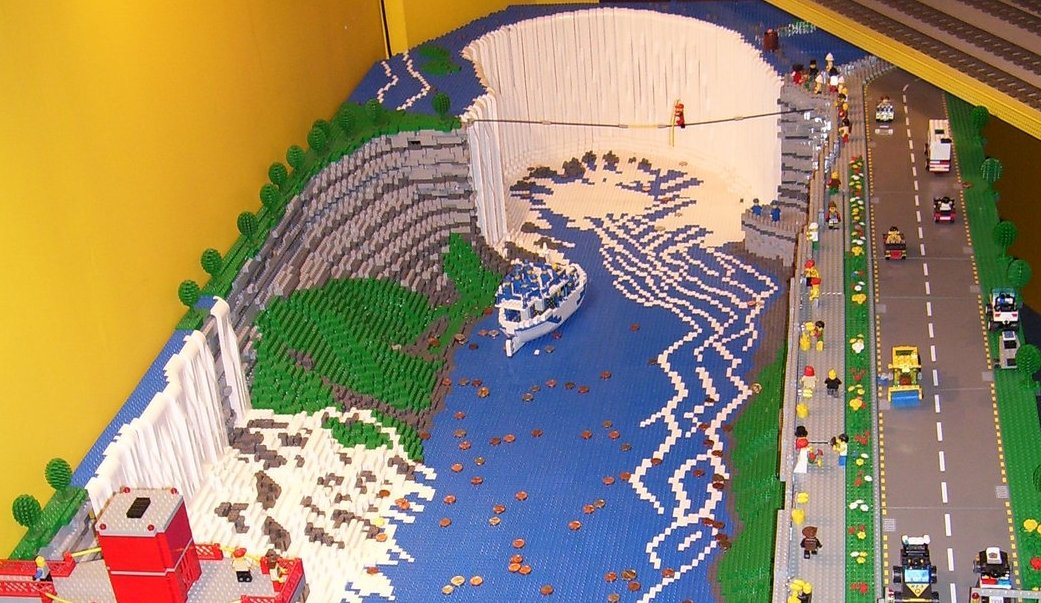
\includegraphics[height=7\baselineskip]{lego}

  \begin{alertbox}{0.9\textwidth}
    Einteilen eines Programms in mehrere Quelldateien    
  \end{alertbox}

  \begin{itemize}
  \item Übersichtlicherer Code
  \item Wiederverwendbarkeit von Teilen des Codes
  \item Schnelleres Neucompilieren bei kleinen Codeänderungen
  \end{itemize}
\end{frame}

\begin{frame}[squeeze,fragile]
  \frametitle{Modularisierung in C}

  \begin{block}{Headerdateien}
    \vspace{-0.5\baselineskip}
    \begin{itemize}
    \item haben üblicherweise Endung "`.h"'
    \item beschreiben, welche Funktionen und Variablen eine Objektdatei/Bibliothek bereitstellt
      (\alert{exportiert})
    \item beschreiben \alert{Signatur} der Funktionen (Typ von Parametern)
    \item beschreiben den Typ von exportierten Variablen
    \end{itemize}
  \end{block}

  \begin{block}{Objektdateien}
    \vspace{-0.5\baselineskip}
    \begin{itemize}
    \item haben üblicherweise Endung "`.o"'
    \item werden wie Progamme aus C-Quellcode erzeugt
    \item oder aus Fortran, Assembler,...-Code
    \item enthalten Programmcode und/oder globale Variablen
    \end{itemize}
  \end{block}

  \begin{itemize}
  \item Namen von Headerdatei und Objektdatei sind unabhängig
  \item \alert{Bibliotheken} sind Sammlungen von Objektdateien
  \end{itemize}
\end{frame}

\begin{frame}[fragile]
  \frametitle{extern und static}
\begin{lstlisting}[emph={extern,static}]
// nur fuer die aktuelle Objektdatei
static char *string1;
// fuer alle sichtbar
       char *string2;
// kommt woanders her
extern char *string3;
\end{lstlisting}

  \begin{onlyenv}<1>
    \begin{itemize}
    \item \emph{globale} Variablen können in mehreren Objektdateien verwendet werden
    \item \lstinline!extern! und \lstinline!static! ändern ihre Sichtbarkeit
    \end{itemize}
  \end{onlyenv}

  \begin{onlyenv}<2>
    {\alerted\bfseries \lstinline!static!} (\lstinline!string1!)
    \begin{itemize}
    \item Platz für diese Variable wird in dieser Objektdatei belegt
    \item Zugriff nur von der aktuellen Objektdatei
    \item Kann daher in mehreren Objektdateien definiert werden
    \item Konstanten sollten daher statisch deklariert werden:
      \lstinline!static const double PI = 3;!
    \end{itemize}
  \end{onlyenv}

  \begin{onlyenv}<3>
    ohne Vorgabe (\lstinline!string2!)
    \begin{itemize}
    \item Platz für diese Variable wird in dieser Objektdatei belegt
    \item Zugriff auch von außen
    \item Darf nur in einer Objektdatei definiert werden
    \item Bei mehrfachem Auftreten gibt der gcc/ld sonst den Fehler
      "`multiple definition of `var'"'
    \item Insbesondere, wenn eine Objektdatei doppelt eingelinkt wird:\\
      \lstinline[language=bash]!gcc -o programm test1.o test1.o!
    \end{itemize}
  \end{onlyenv}

  \begin{onlyenv}<4>
    {\alerted\bfseries \lstinline!extern!} (\lstinline!string3!)
    \begin{itemize}
    \item Platz für diese Variable wird \emph{nicht} in dieser Objektdatei belegt\\
      (wenn keine unqualifizierte Definition folgt)
    \item Diese Variable muss in einer anderen Objektdatei liegen
    \item In genau einer Objektdatei muss diese Variable ohne \lstinline!extern!  definiert werden
    \item Ist die Variable in allen Objektdateien nur extern deklariert, gibt
      gcc/ld den Fehler "`undefined reference to `var'"'
    \end{itemize}
  \end{onlyenv}
\end{frame}

\begin{frame}[fragile]
  \frametitle{Aufbau von Headerdateien}
\begin{lstlisting}[title=modul.h]
#ifndef MODUL_H
#define MODUL_H
// Funktionsdeklaration
const char *funktion();
// Variablendeklaration
extern const char *var;
#endif
\end{lstlisting}

  \begin{itemize}
  \item Der \lstinline!#ifdef/#define!-Kostrukt sichert, dass die Headerdatei modul.h nur einmal
    pro Objektdatei eingebunden wird
  \item Variablen werden hier \lstinline!extern! deklariert
  \item Funktionen werden einfach ohne Funktionskörper deklariert
  \item Variablen und Funktionen müssen in genau einer Objektdatei definiert werden
  \end{itemize}
\end{frame}

\begin{frame}[fragile]
  \frametitle{Aufbau der Quelldateien}
\begin{lstlisting}[title=modul.c]
#include "modul.h"

// die exportierte Funktion
const char *funktion() { return "Hello"; }
// und die exportierte Variable
const char *var = "World";
\end{lstlisting}

  \begin{itemize}
  \item Normaler C-Code wie gehabt, aber i.A. ohne \lstinline!main!
  \item \lstinline!main! muss in genauer einer Objektdatei definiert sein
  \item Üblicherweise bindet man die zugehörige Headerdatei ein
  \item Dadurch fallen Unterschiede in Deklaration und Definition schneller auf
    (z.B. Änderung der Parameter einer Funktion)
  \end{itemize}
\end{frame}

\begin{frame}[fragile]
  \frametitle{Compilieren und Linken}

\begin{lstlisting}[language=bash,emph={c,o}]
# Das Modul modul.o aus modul.c erzeugen
gcc -Wall -O3 -std=c99 @\alerted\bfseries -c@ modul.c

# und main.o aus main.c
gcc -Wall -O3 -std=c99 @\alerted\bfseries -c@ main.c

# programm aus main und modul zusammenbauen
gcc -o programm main.o modul.o
\end{lstlisting}

  \begin{itemize}
  \item C-Quellcode wird mit der Option "`-c"' in Objektdatei übersetzt
  \item Der Compiler verbindet mehrere Objektdateien zu einem Programm
    (\alert{linken})
  \item Tatsächlich ruft er dazu den Linker (ld) auf
  \item make kann benutzt werden, um den Vorgang zu automatisieren
  \end{itemize}
\end{frame}

\begin{frame}[fragile]
  \frametitle{Bibliotheken}

  \begin{itemize}
  \item Statische Bibliotheken sind Archive von Objektdateien
  \item Erzeugen eines Archivs:\\
\begin{lstlisting}[language=bash,emph={ar},style=unframed]
ar rcs libbib.a bib_hello.o bib_world.o
\end{lstlisting}
  \item Linken mit allen Objektdateien in der Bibliothek:
\begin{lstlisting}[language=bash,style=unframed]
gcc main.c  -L. @\alerted\bfseries -lbib@
\end{lstlisting}
  \item Bei Angabe von "`-lbib"' lädt der Compiler automatisch \lstinline[language=bash]!libbib.a!
  \item Mit "`-L"' werden Suchpfade für Bibliotheken angegeben\\
    ("`-L."' = aktuelles Verzeichnis)
  \item Mit \lstinline!nm! lassen sich die definierten Symbole auslesen:
\begin{lstlisting}[language=bash,emph={nm},style=unframed]
nm libbib.a
\end{lstlisting}
\begin{lstlisting}[basicstyle={\fontfamily{fvm}\tiny},language=bash]
bib_hello.o:
0000000000000000 T get_hello
0000000000000000 d hello
      
bib_world.o:
0000000000000000 D world
\end{lstlisting}
\end{itemize}
\end{frame}

\begin{frame}[fragile,squeeze]
  \frametitle{make -- automatisiertes Bauen}
\begin{lstlisting}[language=make,title=Makefile,escapechar={}]
default: bib
libbib.a: bib_hello.o bib_world.o
        ar rcs $@ $^
bib: main.o libbib.a
        gcc -o bib main.o -L. -lbib
clean:
        rm -f bib libbib.a *.o
\end{lstlisting}

  \begin{onlyenv}<1>
    \begin{itemize}
    \item Die Regeldatei muss \lstinline!Makefile! oder \lstinline!makefile! heißen
    \item besteht aus Regeln der Form
\begin{lstlisting}[language=make,escapechar={},style=unframed]
ziel: quelle1 quelle2 ...
       Shell-Befehl
\end{lstlisting}
    \item Shell-Befehl erzeugt aus den Quellen die Datei \lstinline!ziel!
    \end{itemize}
  \end{onlyenv}

  \begin{onlyenv}<2>
    \begin{itemize}
    \item Aufruf einfach mit \lstinline[language=bash]!make ziel!
    \item \lstinline!ziel! wird nur neu gebaut, wenn eine Quelle neuer ist
    \item Bei Bedarf werden auch alle Quellen erneuert
    \item Im Beispiel:
      \begin{itemize}
      \item \lstinline[language=bash]!make default! baut das Programm \lstinline!bib!
      \item \lstinline[language=bash]!make libbib.a! baut nur die Bibliothek \lstinline!libbib.a!
      \end{itemize}
    \end{itemize}
  \end{onlyenv}

  \begin{onlyenv}<3>
    \begin{itemize}
    \item Automatische Regeln für Objektdateien aus C-Quellcode
    \item Beispiel: \lstinline[language=bash]!make bib_hello.o! baut die Objektdatei \lstinline!bib_hello.o!
      aus \lstinline!bib_hello.c!, wenn vorhanden
    \item Regeln ohne Quellen ("`clean"') werden immer ausgeführt
    \item Regeln ohne Befehl ("`default"') erneuern nur die Quellen
    \item Im Beispiel: \lstinline[language=bash]!make default! entspricht \lstinline[language=bash]!make bib!
    \end{itemize}
  \end{onlyenv}
\end{frame}

\begin{frame}
  \frametitle{Pakete selber compilieren}

  \begin{itemize}
  \item Es gibt im WWW eine riesige Menge an Programmpaketen
  \item Meist gibt es Installer bzw. fertige Pakete für die eigene Distribution
  \end{itemize}

  Selber bauen ist aber nötig, wenn
  \begin{itemize}
  \item man keine Root-Rechte hat und der Admin ein Paket nicht installieren will
    (z.B. auf Großrechnern)
  \item es kein fertiges Paket für die Distribution gibt
  \item das fertige Paket ein Feature noch nicht bietet / einen Bug hat
  \item man an dem Paket weiterentwickeln will
  \end{itemize}

  Das geht natürlich nur mit Open-Source-Paketen, wenn ich nicht gerade den Autor kenne!
\end{frame}

\begin{frame}[fragile]
  \frametitle{Linux-Dreisprung}
  
  \begin{itemize}
  \item Die meisten Open-Source-Pakete lassen sich mit drei Befehlen compilieren:
\begin{lstlisting}[language=bash]
./configure

make

make install
\end{lstlisting}
  \item Davor muss das Paket natürlich ausgepackt werden:\\
\begin{lstlisting}[language=bash,style=unframed]
tar -x@\alerted\bfseries z@f paket-1.2.3.tgz!      @\sffamily\normalsize oder@
tar -x@\alerted\bfseries j@f paket-1.2.3.tar.bz2!
\end{lstlisting}
  \item erzeugt normalerweise ein Unterverzeichnis \lstinline!paket-1.2.3!
  \item Skript \lstinline!configure! konfiguriert das Paket zum Bauen,\\
    erzeugt ein Makefile
  \item Wird vom Paket-Maintainer mit Hilfe der GNU-autotools erzeugt
  \end{itemize}
\end{frame}

\begin{frame}[fragile]
  \frametitle{configure}
\begin{lstlisting}[language=bash]
./configure --prefix=WOHIN \
    --with-OPTION --without-OPTION \
    CPPFLAGS="-I$HOME/include" \
    LDFLAGS="-L$HOME/include"
\end{lstlisting}

  \lstinline!configure!-Optionen können variieren, es gibt (fast) immer:
  \begin{onlyenv}<1>
    \begin{itemize}
    \item \lstinline!--help!: beschreibt alle Konfigurationsmöglichkeiten
    \item \lstinline!--prefix!: wohin das Paket installiert werden soll.\\
      Hier einen Platz im eigenen Home-Directory angeben, sonst kann nur root das Paket installieren
    \item \lstinline!--with-OPTION!: schaltet Optionen an (z.B. GUI, Unterstützung für double,...)
    \item \lstinline!--without-OPTION!: schaltet Optionen aus
    \end{itemize}
  \end{onlyenv}

  \begin{onlyenv}<2>
    \begin{itemize}
    \item \lstinline!CPPFLAGS!: Flags für den C-Präprozessor.\\
      Hier kann man weitere Verzeichnisse mit Headerdateien angeben\\
      (\lstinline!CPPFLAGS="-I/my/include -I$HOME/include"!)
    \item \lstinline!LDFLAGS!: Flags für den Linker.\\
      Hier kann man weitere Verzeichnisse mit Bibliotheken angeben
      \\(\lstinline!LDFLAGS="-L/my/lib -L$HOME/lib"!)
    \item Das ist insbesondere bei selbstcompilierten Pakten notwendig
    \item Viele Pakete installieren ein Programm \lstinline!paket-config!, das über die benötigten
      Pfade Auskunft gibt
    \end{itemize}
  \end{onlyenv}
\end{frame}

\begin{frame}[fragile]
  \frametitle{Linux-Dreisprung: make}

  \begin{itemize}
  \item Das Paket wird dann einfach mit \lstinline!make! gebaut
  \item Je nach Komplexität kann das auch mal Stunden dauern...
  \item Tipp:\\
    {\alerted\lstinline!make -j N!}\\
    compiliert N Objektdateien gleichzeitig
  \item Ist der Computer nicht anderweitig belastet, ist es am schnellsten, wenn N der doppelten
    Anzahl der Prozessor-Kerne entspricht
  \item Auf einem Quadcore also \lstinline!make -j 8!
  \item \lstinline!make install! installiert das compilierte Paket
    \begin{itemize}
    \item Ausführbare Dateien landen in \lstinline!PREFIX/bin!
    \item Bibliotheken in \lstinline!PREFIX/lib!
    \item Headerdateien in \lstinline!PREFIX/include!
    \item Hilfedateien in \lstinline!PREFIX/share/man/man*!
    \end{itemize}
  \end{itemize}
\end{frame}

\begin{frame}
  \frametitle{Beispiele nützlicher Bibliotheken für C}
  \begin{itemize}
  \item GSL -- GNU Scientific Library\\
    \url{http://www.gnu.org/software/gsl}\\
    \begin{itemize}
    \item viele Zufallszahlengeneratoren
    \item Spezielle Funktionen (Bessel-, Gammafunktion, ...)
    \item Auswertetools (Statistik, Histogramme, ...)
    \end{itemize}
  \item FFTW -- Fastest Fourier Transform in the West\\
    \url{http://www.fftw.org}
  \item GTK für graphische Interfaces à la GIMP, GNOME, XFCE, ...\\
    \url{http://www.gtk.org}
  \item Open MPI, eine MPI-Implementation für viele Plattformen\\
    \url{http://www.open-mpi.org}
  \end{itemize}
\end{frame}

\end{document}

%%% Local Variables:
%%% mode: latex
%%% TeX-PDF-mode: t
%%% TeX-master: t
%%% fill-column: 100
%%% End:
